\section{ANÁLISE DO SISTEMA}

Aplicação dos conceitos da TGS ao sistema escolhido no caso o \textbf{TikTok}, detalhando cada aspecto listado na metodologia.

\subsection{Objetivo do Sistema}

O TikTok tem como objetivo fundamental a criação e compartilhamento de vídeos curtos, proporcionando um espaço no qual os usuários podem se expressar de maneira dinâmica e criativa.\vskip0.3cm 

A plataforma oferece diversas ferramentas de edição e aprimoramento de vídeos, permitindo que os conteúdos sejam personalizados e atrativos. Além desse objetivo central, o TikTok incorpora um conjunto de outros propósitos interligados, tais como:


\begin{itemize}
    \item \textbf{Entretenimento e Diversão}: O TikTok visa oferecer momentos de lazer por meio de vídeos curtos, desafios virais e tendências populares, mantendo os usuários engajados na plataforma.
    \item \textbf{Engajamento e Interação Social}: A plataforma fomenta a interação entre os usuários, criando um ambiente altamente participativo, no qual é possível curtir, comentar e compartilhar conteúdos.
    \item \textbf{Expressão Criativa}: Com recursos avançados de edição, trilhas sonoras, filtros e efeitos especiais, o TikTok incentiva a produção de conteúdos inovadores, permitindo que os usuários explorem sua criatividade.
    \item \textbf{Viralização e Disseminação de Conteúdo}: O algoritmo da plataforma favorece a viralização rápida dos vídeos, potencializando a propagação de desafios, trends e conteúdos de grande alcance.
    \item \textbf{Educação e Informação}: Além do entretenimento, o TikTok também se tornou um canal para a disseminação de conhecimento, oferecendo conteúdos educativos, tutoriais e informações sobre diversos temas.
\end{itemize}


Diante dessas características, observa-se que o TikTok atrai predominantemente um público jovem-adulto, impulsionado pelos seguintes fatores:


\begin{itemize}
    \item O formato de vídeos curtos facilita o consumo rápido e dinâmico de conteúdos.
    \item O algoritmo de recomendação personaliza a experiência do usuário com base em suas interações.
    \item As ferramentas de edição possibilitam a criação de conteúdos cada vez mais sofisticados e atrativos.
    \item O engajamento ocorre por meio de curtidas, compartilhamentos, comentários e reações.
     \item A cultura de desafios e trends incentiva a participação ativa e a reprodução de conteúdos.
\end{itemize}


Dessa forma, conclui-se que o TikTok não possui um único objetivo central, mas se destaca principalmente por promover o entretenimento e o engajamento, sendo esses os aspectos mais evidentes em seu funcionamento.

\newpage
\subsection{Entradas (Inputs) do Sistema}

Segundo Conceição et al (2024), para formalizar o processo de obtenção dos dados, existe um momento de assinatura do contrato do serviço entre as partes, e o usuário é instado a formalizar o aceite antes mesmo da utilização.\vskip0.3cm


As entradas no sistema representam os recursos e informações que alimentam o TikTok. Essas entradas incluem:


\subsection{Dados do Usuário}

Esses dados ajudam a definir o perfil do usuário, permitindo que o TikTok ofereça conteúdo mais direcionado com base na sua identidade e nas suas preferências. 

\begin{itemize}
    \item \textbf{Nome}: O nome do usuário é coletado quando ele se registra no aplicativo. O nome pode ser fornecido diretamente pelo próprio usuário ao criar uma conta, seja por meio do login com uma rede social (como Facebook, Instagram, etc.) ou por meio do preenchimento manual;
    \item \textbf{Idade}: a idade é coletada durante o processo de registro, onde o usuário precisa fornecer sua data de nascimento. O TikTok, por motivos legais e para a criação de uma experiência apropriada à faixa etária, é solicitar essa informação.
    \item \textbf{Gênero}: o gênero é coletado no momento do registro, quando o usuário é solicitado a fornecer essa informação de forma opcional. Essa coleta é muitas vezes realizada por meio de uma caixa de seleção (masculino, feminino, outro) ou pode ser inferida a partir do nome de usuário, fotos e outros dados, embora essa prática possa ser limitada em algumas regiões.
    \item \textbf{Localização Geográfica}: a localização do usuário é coletada por meio de dados de geolocalização do dispositivo, quando o usuário dá permissão para o TikTok acessar a sua localização. Isso pode ser feito por meio do GPS do celular, o endereço IP ou Wi-Fi utilizado.
    \item \textbf{Idioma}: o idioma é coletado diretamente do dispositivo, pois a maioria dos dispositivos móveis define o idioma de exibição com base nas configurações de idioma do sistema;
    
    \newpage
    \item \textbf{E-mail}: O e-mail é geralmente coletado no momento do registro ou criação da conta, onde o usuário é solicitado a fornecer um endereço de e-mail válido. O TikTok pode pedir ao usuário para verificar o e-mail, enviando um código de confirmação para garantir que a conta seja associada a um e-mail legítimo.
    \item \textbf{Número de Telefone}: O número de telefone é solicitado como uma opção durante o processo de registro ou de verificação de conta. O TikTok pode pedir ao usuário para fornecer o número de telefone para ativar uma camada extra de segurança, ou para possibilitar a recuperação de conta em caso de problemas com a senha. A verificação do número é realizada através de um código enviado por SMS.
    \item \textbf{Senha}: A senha é criada pelo usuário durante o processo de registro, onde ele escolhe uma senha pessoal para proteger a conta. O TikTok exige que a senha tenha um nível mínimo de complexidade (como uma combinação de letras, números e caracteres especiais) para aumentar a segurança.
\end{itemize}



\subsection{Dados de Postagem}

Os dados de postagem no TikTok são fundamentais para o funcionamento do algoritmo de recomendação e para medir o engajamento de um usuário com o conteúdo na plataforma. Aqui está uma explicação detalhada de como cada tipo de dado é coletado e utilizado:

\begin{itemize}
    \item \textbf{Videos}: Cada vez que o usuário publica um vídeo, o TikTok coleta informações sobre o vídeo, como o conteúdo visual, áudio, hashtags, legendas, e efeitos aplicados. Além disso, o algoritmo rastreia como o vídeo é recebido pelos outros usuários (curtidas, comentários, compartilhamentos, etc.);
    \item \textbf{Curtidas}: O TikTok registra todas as curtidas que um vídeo recebe, assim como as curtidas feitas pelos usuários nos vídeos de outros. Cada vez que o usuário clica no ícone de "curtir" em um vídeo, esse dado é coletado;
    \item \textbf{Comentários}: O TikTok coleta os comentários feitos nos vídeos, bem como os comentários feitos por um usuário em vídeos de outras pessoas. Isso inclui o texto dos comentários e a interação com esses conteúdos;
    \item \textbf{Compratilhamento}: O TikTok registra todas as vezes que um vídeo é compartilhado. Isso inclui o compartilhamento dentro da própria plataforma (enviar para amigos, grupos, etc.) e para fora da plataforma (compartilhar em outras redes sociais ou via mensagem);
    \item \textbf{Tempo de Visualização}: O TikTok monitora quanto tempo um usuário passa assistindo a cada vídeo. Isso inclui o tempo total de visualização e se o usuário assistiu ao vídeo inteiro ou pulou partes dele. Esses dados são coletados automaticamente enquanto o vídeo é exibido;
    \item  \textbf{Buscas Realizadas}: O TikTok coleta as pesquisas realizadas pelos usuários dentro da plataforma, incluindo termos de busca, usuários seguidos, hashtags, músicas e conteúdos específicos;
    \item \textbf{Seguidores}: O TikTok registra o número de seguidores de cada usuário, assim como as interações dos usuários com os perfis de outros, como o ato de seguir ou deixar de seguir;
    \item  \textbf{Visitas no Perfil}: O TikTok rastreia o número de visitas que um perfil recebe. Isso inclui as visitas feitas por pessoas que já seguem o usuário e por aquelas que não seguem, além de monitorar se o perfil é visitado frequentemente ou esporadicamente.
\end{itemize}



\newpage
\subsection{Processos do Sistema}

O sistema do TikTok transforma entradas (dados de usuários e conteúdo) em saídas (recomendações personalizadas, feed ajustado e ações realizadas na plataforma) por meio de um conjunto de processos complexos que envolvem algoritmos, ferramentas e infraestrutura tecnológica. \vskip0.3cm

O TikTok realiza diversos processos internos para transformar entradas em saídas:

\begin{itemize}
    \item \textbf{Processamento e Armazenamento de Dados}: o algoritmo de recomendação processa dados de uso em tempo real utilizando ferramentas de Big Data e Armazenamento em Nuvem, identificando padrões de comportamento e preferências dos usuários.
    \item \textbf{Classificação de Conteúdo}: os vídeos são analisados utilzando Redes Neurais Profundas, com base em hashtags, tendências e elementos visuais para categorização e promoção.
    \item \textbf{Personalização e Recomendações}: o feed “For You” é ajustado continuamente para apresentar conteúdo relevante para cada usuário, usando redes neurais recorrentes para prever o interesse de um usuário em cada vídeo.
    \item \textbf{Moderação de Conteúdo}: Processos de verificação automática e humana são usados para identificar e remover conteúdo inadequado ou que viole os termos da plataforma.
    \item \textbf{Otimização Técnica}: Melhorias de desempenho do aplicativo, como tempo de carregamento e estabilidade.
\end{itemize}


\newpage
\subsection{Saídas (Outputs) do Sistema}

\subsection{Monetização}

Atualmente, há alguns modos de monetização Direta pelo Tiktok (CATUCCI et al, 2023).

\subsubsection{Requesitos para Monetização}

Os principais requisitos para a monetização no Tiktok.

\begin{enumerate}
    \item \textbf{Idade Mínima de 18 Anos}: Para participar do programa de monetização do TikTok, é necessário ter pelo menos 18 anos de idade. Isso garante que os usuários sejam legalmente capazes de gerenciar seus ganhos e cumprir com as obrigações fiscais associadas;
    \item \textbf{10 Mil Seguidores}: Umn número significativo de seguidores é essencial para garantir que seu conteúd oalcance uma audiência ampla eengajada. Com 10 milseguidores, você demonstra uma base sólida de apoio e interesse em seu conteúdo, tornando-o elegível para a monetização;
    \item \textbf{100 Mil Views nos Últimos 30 Dias}: Além de te rseguidores, é crucial que seu conteúdo seja visualizado por um grande número de pessoas. Alcançar 100 mil views nos últimos 30 dias indica que seu conteúdo é popular e tem potencial para gerar receita por meio de anúncios e outras oportunidadesde monetização;
    \item \textbf{Vídeos com Mais de Um Minuto de Duração}: Para serem qualificados para a monetização através do programa criativo do TikTok, seus vídeos precisam ter uma duração mínima de um minuto. Isso garante ques eu conteúdo tenha espaço suficiente para atrair e reter a atenção do público, aumentando suas chancesde gerar receita Após cumprir esses requisitos, você estaráqualificado para solicitar a entrada no programa demonetização do TikTok. Este processo envolve preencher algumas informações fiscais e aguardar aaprovação do TikTok.Uma vez aprovado, você estará pronto para começara monetizar seu conteúdo e dar o próximo passo em sua jornada de criação de conteúdo online.
    \end{enumerate}


\subsubsection{Tipos para Monetização}

\begin{enumerate}
    \item \textbf{Programa de monetização TikTok Creator Fund}: Os criadores podem ganhar dinheiro com o TikTok por meio do Creator Fund, um fundo de monetização para criadores com pelo menos 100.000 visualizações em 30 dias. O pagamento varia com base no desempenho dos vídeos.

\item \textbf{Convide Seus Amigos}: Um dos meios mais comuns de faturar uma grana no TikTok é convidar os seus amigos para ingressar na plataforma — estratégia da própria empresa para expandir o seu número de inscritos. Quanto mais pessoas conseguir levar para o TikTok, mais moedas você ganha, e elas podem ser trocadas por recompensas em dinheiro.

\item \textbf{Cumpra Missões Diárias}: O TikTok permite que você cumpra missões diárias para ganhar rubis, pontos que podem ser trocados por dinheiro ou benefícios. Cada unidade de rubi equivale a R\$ 0,00001. Por exemplo, se você acumular 10 mil rubis, poderá embolsar o equivalente a R\$ 1.

\item \textbf{Lives}:
Você pode fazer lives no TikTok e ganhar moedas com base no tempo de transmissão, podendo arrecadar mais de mil rubis se o seu vídeo durar aproximadamente meia hora — tempo recomendado pela própria rede social.


\item \textbf{Afiliados}: Você pode usar link de afiliados para monetizar o TikTok, inserindo endereços clicáveis em seus vídeos e na sua bio — no melhor estilo Instagram. Esses links podem redirecionar para sites de vendas de produtos, serviços e demais categorias que se encaixem no programa de afiliados do TikTok e possam render alguma comissão.

\end{enumerate}




Após cumprir esses requisitos, o usuário estará qualificado para solicitar a entrada no \textbf{Programa de Monetização} do Tiktok. Este Processo envolve prencher algumas informações fiscais e aguardar a aprovação do Tiktok.















\subsection{SubSistemas}

O algoritmo de recomendação do TikTok é um dos elementos centrais para sua popularidade global. Ele utiliza uma combinação de dados de engajamento, preferências dos usuários, informações do conteúdo e desempenho inicial para oferecer um feed personalizado. Cada interação do usuário, como curtidas, comentários e compartilhamentos, contribui para a identificação de interesses específicos. As preferências também são refinadas com base no tipo de conteúdo assistido e no tempo de visualização. Além disso, o algoritmo valoriza conteúdos originais e relevantes para tendências atuais, utilizando metadados como hashtags e descrições para categorização. Vídeos recém-publicados passam por testes iniciais com públicos pequenos antes de serem amplamente distribuídos, dependendo do engajamento gerado. A frequência de publicação e a consistência na qualidade do conteúdo também influenciam na visibilidade. Esses processos, apoiados por sistemas de inteligência artificial, garantem que os usuários recebam uma experiência única e imersiva na plataforma.


\newpage

\subsubsection{Subsistema de Captura e Edição de Vídeos}

Para criar e editar vídeos no Tiktok, atualmente, existem vários recursos fáceis de aplicar. Você pode gravar um vídeo “em tempo real” de dentro do aplicativo TikTok ouselecionar um vídeo criado anteriormente e editá-lo antes de postá-lo. \vskip0.3cm

Abra o aplicativo TikTok. Você verá um ícone “+” na barra de menu na parte inferior da tela. Toque aqui e você irá para a tela de gravação.\vskip0.3cm

Você pode configurar vários recursos antes de começar a gravar seu vídeo. O recurso “Timer” é muito útil para gravação de vídeo sem as mãos. Você também pode escolher entre os vários filtros e efeitos de beleza e, quando fizer suas escolhas, estará pronto para começar a gravar seu vídeo.\vskip0.3cm

Agora você precisa selecionar a duração do seu vídeo como\textbf{ 15 ou 60 segundos ou 10 minutos}. Há um grande botão vermelho redondo na parte inferior da tela e quando você tocar nele, sua gravação será iniciada.\vskip0.3cm

Quando terminar a gravação, é altamente recomendável que você escolha alguma música de fundo. Você verá um catálogo de clipes de música à sua escolha. Todos esses são clipes curtos que você pode adicionar ao seu vídeo.



\begin{figure}[H]
    \centering
    \begin{minipage}{0.45\textwidth}
        \centering
        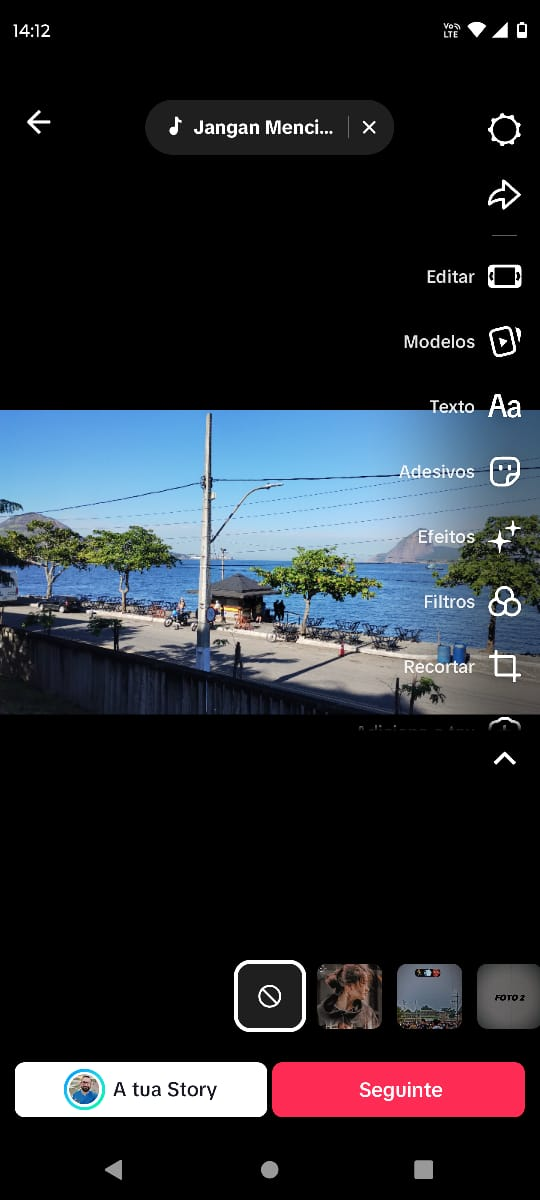
\includegraphics[width=\linewidth]{Relatório/Figuras/edicao_video1.jpeg}
        \caption{Tela do app TikTok, chamada "\textbf{Verificar Conta}", Fazendo Análise de Cada Vídeo e Imagem.}
        \label{fig:promover_publicacao1}
    \end{minipage}\hfill
    \begin{minipage}{0.45\textwidth}
        \centering
        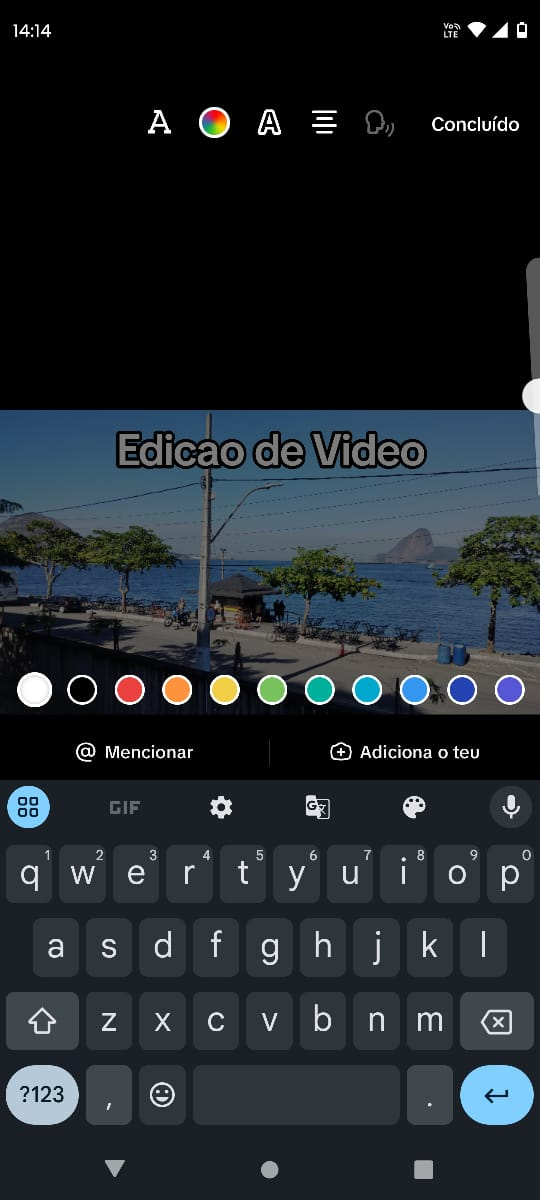
\includegraphics[width=\linewidth]{Relatório/Figuras/edicao_video2.jpeg}
        \caption{Tela do app TikTok, chamada "\textbf{Verificar Conta}", Análise Final, Conta Regular.}
        \label{fig:promover_publicacao2}
    \end{minipage}
\end{figure}







\newpage
\subsubsection{Subsistema de Verificação de Conta}


\begin{figure}[H]
    \centering
    \begin{minipage}{0.45\textwidth}
        \centering
        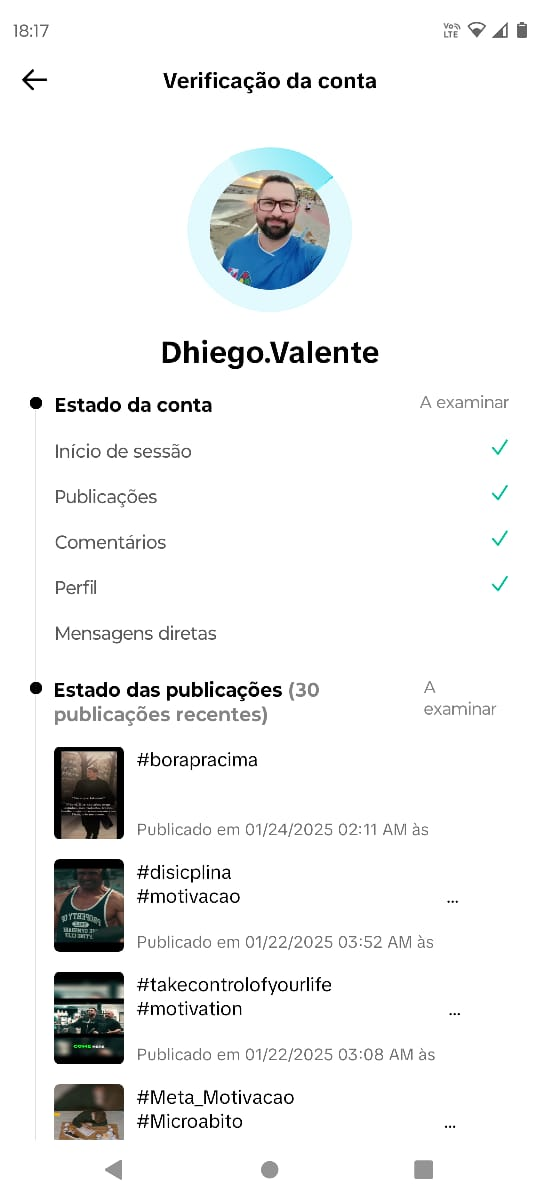
\includegraphics[width=\linewidth]{Relatório/Figuras/verificacao_conta1.jpeg}
        \caption{Tela do app TikTok, chamada "\textbf{Verificar Conta}", Fazendo Análise de Cada Vídeo e Imagem.}
        \label{fig:promover_publicacao1}
    \end{minipage}\hfill
    \begin{minipage}{0.45\textwidth}
        \centering
        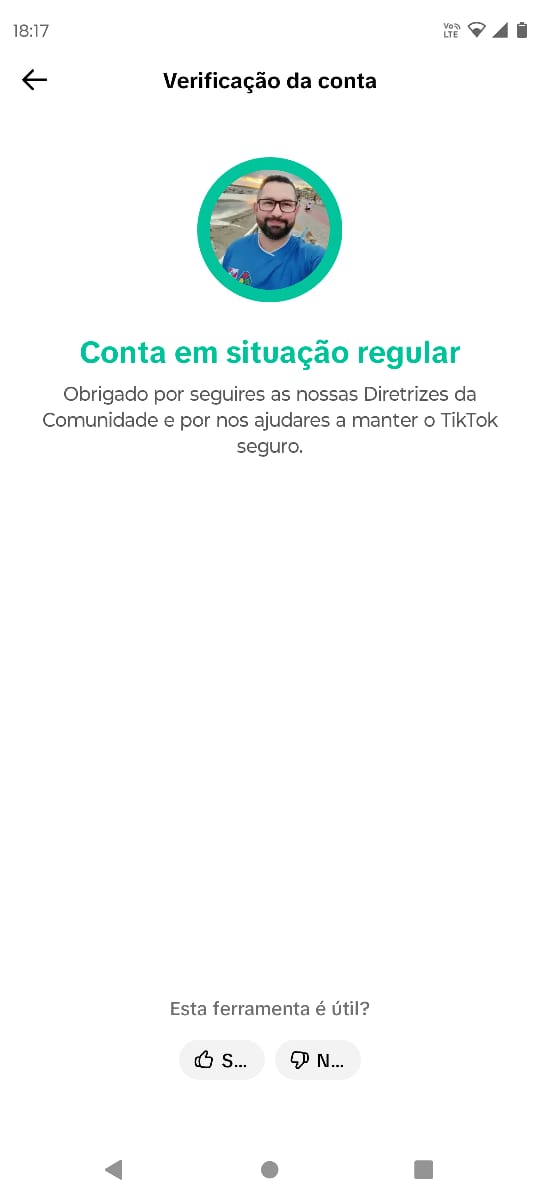
\includegraphics[width=\linewidth]{Relatório/Figuras/verificacao_conta2.jpeg}
        \caption{Tela do app TikTok, chamada "\textbf{Verificar Conta}", Análise Final, Conta Regular.}
        \label{fig:promover_publicacao2}
    \end{minipage}
\end{figure}













\newpage
\subsubsection{Subsistema de Moderação de Conteúdo}










\newpage
\subsubsection{Subsistema de Análise de Dados}

O subsistema de dados e análise é responsável pela coleta, processamento e análise dos dados gerados pelas interações dos usuários na plataforma.\vskip0.3cm


Os insights mais abrangentes que o TikTok oferece são para vídeos. Na sub aba, “\textbf{Visão Geral}”, você encontrará um gráfico de barras que exibe as visualizações dos vídeos nos últimos 7 dias (default). Porém, podendo ser personalizada, escolhendo os últimos 28, 60 e 365 dias.


\begin{figure}[H]
    \centering
    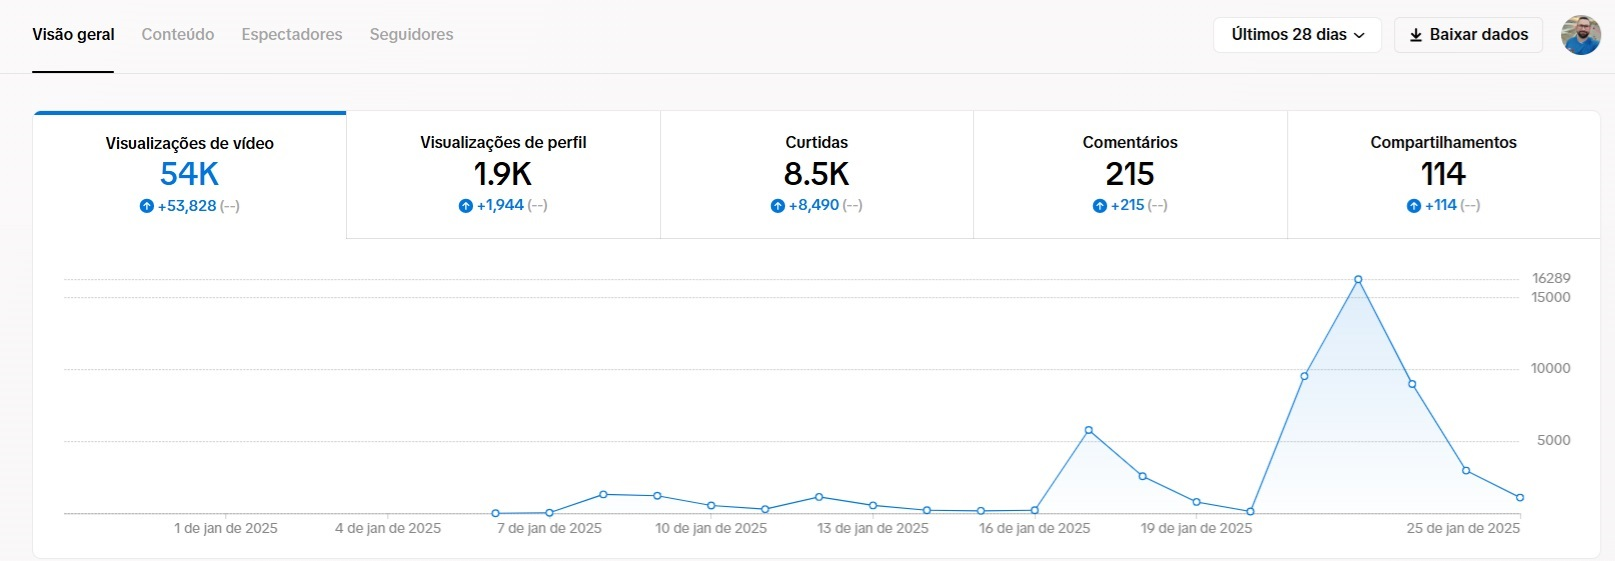
\includegraphics[width=1\linewidth]{Relatório/Figuras/analise_video1.jpg}
    \caption{Tela do Subsistema de “Análise Dados” no app Tiktok, chamada “\textbf{Visão Geral}”.}
    \label{fig:enter-label2} 
\end{figure}

O dashboard mostrado na figura \ref{fig:enter-label2}, apresenta diversas métricas sobre os vídeos postados pelo usuário. A primeira parte é o número de vezes que os espectadores assistiram aos seus vídeos(+- 59.000 views). A segunda é o número de vezes que seu perfil foi visitado(+- 1.900 vezes). A terceira parte é composta pelo número de Curtidas, Comentários e Compartilhamentos.

\newpage
Na sub aba, “Conteúdo”, você visualiza as 10 maiores publicações com melhor desempenho nos últimos 7 dias (default), classificadas de acordo com visualizações (views).\vskip0.3cm

Sendo possível clicar em cada publicação, e verificar o tempo médio que os espectadores passaram assistindo, o percentual que viu o vídeo completo, e o número de usuários que começaram a seguir você, a taxa de retenção, a origem do tráfego e os países ou regiões .



\begin{figure}[H]
    \centering
    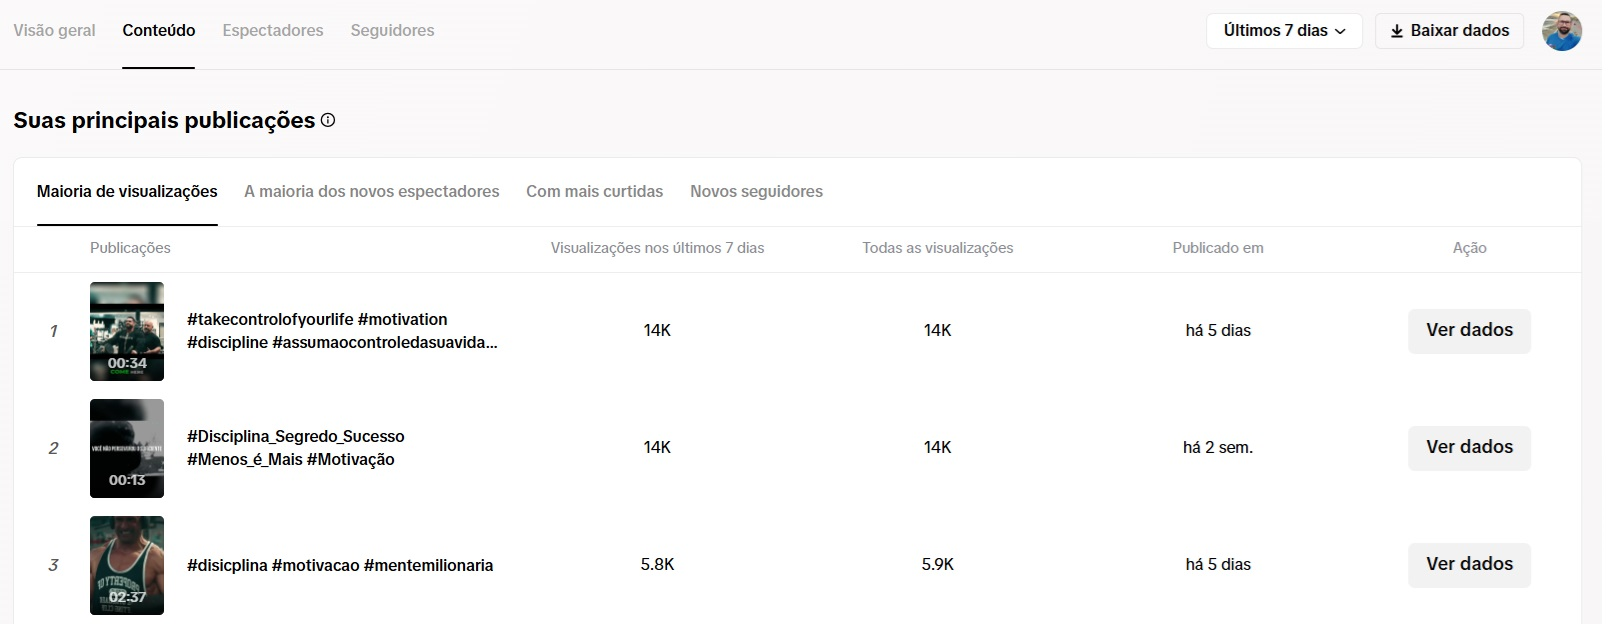
\includegraphics[width=1\linewidth]{Relatório/Figuras/analise_video2.jpg}
    \caption{Tela do Subsistema de “Análise Dados” no app Tiktok, chamada “\textbf{Conteúdo}”}
    \label{fig:enter-label} 
\end{figure}

\newpage
\subsubsection{Subsistema de Promover Publicação}

O Promover é uma ferramenta de publicidade que pode ajudar você a aumentar o engajamento e a visibilidade de suas publicações no TikTok, promovendo seu conteúdo normalmente como um anúncio (TIKTOK, 2023a).



\begin{figure}[H]
    \centering
    \begin{minipage}{0.45\textwidth}
        \centering
        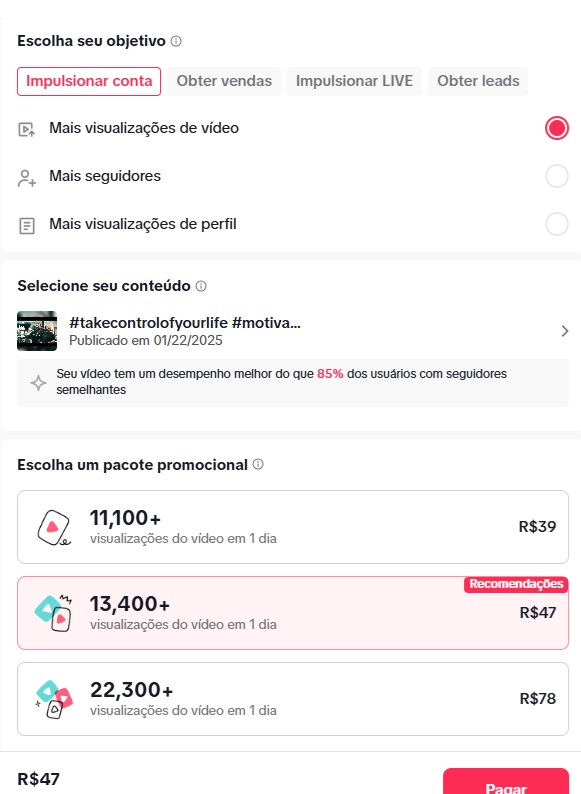
\includegraphics[width=\linewidth]{Relatório/Figuras/promover_publicação1.jpg}
        \caption{Tela do app TikTok, chamada "\textbf{Promover Publicações}" (impulsionar visualização de vídeos).}
        \label{fig:promover_publicacao1}
    \end{minipage}\hfill
    \begin{minipage}{0.45\textwidth}
        \centering
        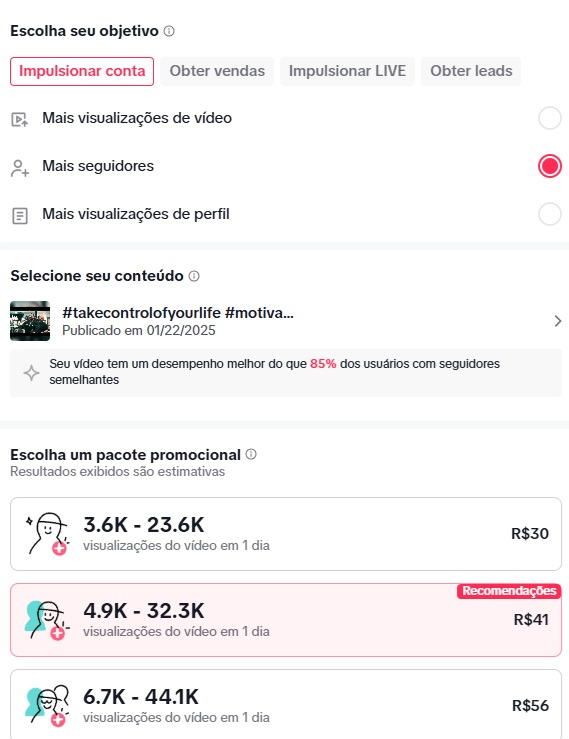
\includegraphics[width=\linewidth]{Relatório/Figuras/promover_publicação2.jpg}
        \caption{Tela do app TikTok, chamada "\textbf{Promover Publicações}" (impulsionar mais seguidores).}
        \label{fig:promover_publicacao2}
    \end{minipage}
\end{figure}










\newpage
\subsection{Fronteiras do Sistemas}





\subsection{Retroalimentação do Sistema}

A  retroalimentação é primordial para o bom funcionamento dos sistemas, e no tiktok  por conta de seu algoritmo de recomendação existem dois tipos de retroalimentações, sendo a positiva(ocorre quando uma ação no sistema gera uma resposta que reforça ou amplifica esse comportamento, tornando-o mais frequente) e negativa (acontece quando uma ação no sistema gera uma resposta que reduz ou limita determinado comportamento), na positiva destacam-se:

\begin{itemize}
 \item \textbf{Viralização de Vídeos}: Quanto mais um vídeo recebe curtidas, comentários e compartilhamentos, mais ele é recomendado pelo algoritmo, aumentando seu alcance.
\item \textbf{Engajamento Aumentado pelo Algoritmo}: Se um usuário assiste a vídeos de um determinado tema (ex: dança, humor, tecnologia), o TikTok passa a recomendar mais conteúdos similares, incentivando o usuário a continuar assistindo.
\item \textbf{Tendências e Desafios Virais}: Quando um desafio (challenge) ou trend ganha popularidade, mais usuários participam, criando novos vídeos e reforçando ainda mais a tendência.
\item \textbf{Uso de Áudios Populares}: Músicas e sons que são utilizados em muitos vídeos aparecem com mais destaque, incentivando outros criadores a usá-los, o que aumenta ainda mais a popularidade do áudio.
\item \textbf{Interações Entre Usuários}: Se um vídeo recebe muitos comentários e respostas, o TikTok pode recomendá-lo para mais pessoas, incentivando ainda mais interações.
\item \textbf{Criadores de Conteúdo Ganhando Mais Visibilidade}: Quanto mais um criador recebe engajamento, mais seus vídeos aparecem para novos usuários, aumentando sua base de seguidores.
\item \textbf{Tempo de Permanência na Plataforma}:
O algoritmo aprende o que mantém os usuários assistindo por mais tempo e ajusta as recomendações para aumentar a retenção na plataforma.
\item \textbf{Efeito "For You" (Para Você)}:
Se um vídeo recebe muitas interações logo após ser postado, ele entra na aba "Para Você" demais usuários, aumentando ainda mais sua visibilidade.
\end{itemize}


Com isso, a retroalimentação positiva do TikTok impulsiona a viralização de vídeos, tendências e engajamento, tornando a plataforma dinâmica e viciante para os usuários.\vskip0.3cm

Já na retroalimentação negativa no TikTok, como destacada anteriormente, ocorre quando uma ação gera uma resposta que reduz, limita ou corrige determinado comportamento, evitando excessos e equilibrando o sistema; assim, nessa retroalimentação destacam-se:

\begin{itemize}
\item \textbf{Remoção de Conteúdos Inadequados}:
Vídeos que violam as diretrizes da comunidade (como discurso de ódio, fake news ou violência) são removidos ou recebem restrição de alcance.

\item \textbf{Redução do Alcance de Vídeos Pouco Interativos}:
Se um vídeo não recebe curtidas, comentários ou compartilhamentos, o TikTok para de recomendá-lo, reduzindo sua visibilidade.

\item \textbf{Despriorização de Conteúdos Repetitivos}:
Se um usuário assiste repetidamente ao mesmo tipo de vídeo sem interagir com novos conteúdos, o algoritmo pode variar as recomendações para evitar que ele perca interesse na plataforma.

\item \textbf{Bloqueio ou Restrição de Contas}:
Contas que recebem muitas denúncias por comportamento inadequado podem ser restringidas ou banidas da plataforma.

\item \textbf{Controle de Spam}: 
Comentários considerados spam (como excesso de emojis ou links repetidos) podem ser ocultados automaticamente.

\item \textbf{Penalização de Vídeos Denunciados}:
Se um vídeo recebe muitas denúncias, ele pode ser removido automaticamente ou revisado manualmente pela equipe do TikTok.

\item \textbf{Filtragem de Conteúdos Sensíveis}:
Conteúdos considerados sensíveis (como imagens chocantes) podem ser sinalizados com avisos ou ocultados de menores de idade.
\end{itemize}



Assim, podemos analisar que ambas as retroalimentações são fundamentais para proporcionar uma experiência confortável aos usuários, garantindo um ambiente seguro e dinâmico. A retroalimentação positiva impulsiona conteúdos populares, ampliando o engajamento, enquanto a negativa filtra e limita materiais inadequados. Dessa forma, o sistema de recomendação do TikTok ajusta continuamente os conteúdos exibidos com base nas interações dos usuários, equilibrando a popularidade e a segurança da plataforma. Isso contribui para a relevância do aplicativo, tornando-o um espaço atraente e confiável para os usuários.




\subsection{Interdepenências com Outros Sistemas}